\begin{frame}{Data Explanation}
\begin{itemize}
 \item 1514 MD Anderson patients who had brain mets from breast cancer between October 2009 and 
 December 2012
 \item 1242 usable cases
 \item 90 covariates
 \begin{itemize}
  \item Missingness from 0 to 65\%
 \end{itemize}

\end{itemize}
\begin{table}[!ht]
\centering
\begin{tabular}{|c|c|}
\hline
Type                                                                            & Example                                                                       \\ \hline
Subject data                                                                    & Age range, race, date of birth                                                \\ \hline
Breast Cancer data                                                                     & TNM staging, type, receptor status                                            \\ \hline
\begin{tabular}[c]{@{}c@{}}Pre brain mets\\ data\end{tabular}                   & Treatment types                                                               \\ \hline
\begin{tabular}[c]{@{}c@{}}Post brain mets\\ clinical observations\end{tabular} & Seizures, headache, nausea                                                    \\ \hline
\begin{tabular}[c]{@{}c@{}}Post brain mets\\ data\end{tabular}                  & \begin{tabular}[c]{@{}c@{}}Treatment type, \\ type of brain mets\end{tabular} \\ \hline
Survival data                                                                   & Survival time after brain mets, censoring indicator                           \\ \hline
\end{tabular}
\caption{Data Categories and Examples}
\label{table:cats}
\end{table}

\end{frame}

\begin{frame}{Questions of interest}
Want to explore...
\begin{itemize}
 \item Chemotherapeutic drugs: Capecitabine vs other chemotherapeutic agents
 \item HER2 directed therapies (Lapatinib, Trastuzumab) in HER2+ subjects
 \item Note: treatment not determined at time of diagnosis, need to landmark (2 months)
 
 \note{Human epidermal growth factor receptor 2 (HER2) overexpression drives the biology of 20
 pct of breast cancers, and predicts a poor prognosis for patients.}
\end{itemize}

 
\end{frame}


\begin{frame}{Important Covariates}
 \begin{table}[ !ht]
\centering
\adjustbox{max height=\dimexpr\textheight-5.5cm\relax,
           max width=\textwidth}{
\begin{tabular}{|c|c|c|}
\hline
Name        & \begin{tabular}[c]{@{}c@{}}Percent \\ Missing\end{tabular} & Meaning                                                                                                                                             \\ \hline
hrher2      & 5                                                        & \begin{tabular}[c]{@{}c@{}}Categorical variable: The hormonal receptor and \\ HER2 receptor status of the subject\end{tabular}                      \\ \hline
agebrainmet & 0                                                          & Indicator: Age greater or less than 60 at time of brain mets                                                                                        \\ \hline
timedx      & 1                                                         & \begin{tabular}[c]{@{}c@{}}Indicator: Time (years) from breast cancer diagnosis to brain\\ mets diagnosis greater or less than 6 years\end{tabular} \\ \hline
site5       & 1                                                        & Indicator: First metastasis was to brain                                                                                                            \\ \hline
race2       & 0                                                          & Categorical: White, Black, Hispanic, other                                                                                                          \\ \hline
priorn      & 0                                                          & \begin{tabular}[c]{@{}c@{}}Indicator: Number of prior treatments in metastatic setting \\ before brain mets\end{tabular}                            \\ \hline
braintype   & 4                                                        & Categorical: Single, multiple, Leptomeningeal disease                                                                                               \\ \hline
controlled  & 12                                                        & Indicator: Extracranial progression of brain mets                                                                                                   \\ \hline
capeothno   & 18                                                        & \begin{tabular}[c]{@{}c@{}}Indicator: Capecitabine, other, or no chemotherapeutic\\ treatment. Treatment variable 1\end{tabular}                     \\ \hline
lapatrasno  & 18                                                        & \begin{tabular}[c]{@{}c@{}}Indicator: Lapatinib, Trastuzumab, or no HER2 treatment.\\ Treatment variable 2\end{tabular}                             \\ \hline
os          & 0                                                          & Overall survival (months)                                                                                                                           \\ \hline
dead        & 0                                                          & Indicator: death indicator                                                                                                                          \\ \hline
her2        & 10                                                        & Indicator: HER2 receptor status                                                                                                                     \\ \hline
\end{tabular}
}
\caption{Table of important covariates to be used in the analysis}
\label{table:importantvars}

\end{table}
\end{frame}

\begin{frame}{Visualization of Missingness}
 \begin{figure}[h!]
  \centering
    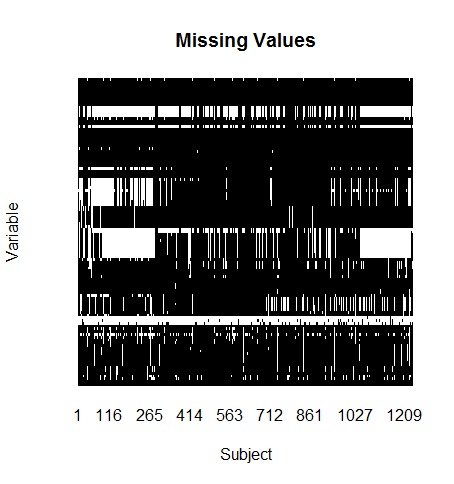
\includegraphics[width=0.8\textwidth]{missingvalues_plot.png}
  \caption{Visualization of missingness in the cancer dataset}
\label{fig:missingplot}

\end{figure}
\end{frame}

\begin{frame}{Imputation}
 \begin{itemize}
  \item MAR assumption seems reasonable
  \item FCS over JM due to nature of data
  \item Need to set up models and predictors
  \item Check for convergence and validity
 \end{itemize}

\end{frame}

%issues were here


\begin{frame}{Convergence}
 
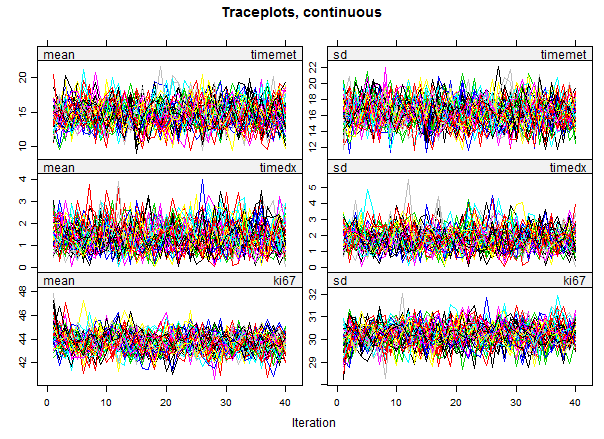
\includegraphics[width=.5\textwidth]{traceplots1}%
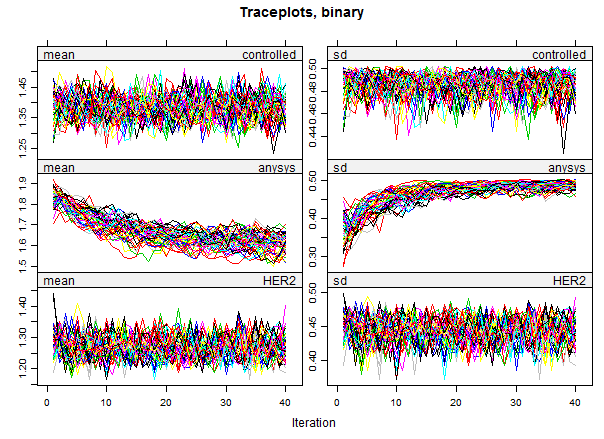
\includegraphics[width=.5\textwidth]{traceplots2} 

\note{On convergence, the different streams should be freely intermingled with one another,
without showing any definite trends. Convergence is diagnosed when the variance between different 
sequences is no larger than the variance within each individual sequence.
We do mean, because without it, we would have 50*missing num for each
var, and it would be very hard to read}

\end{frame}

\begin{comment}
 
\begin{frame}{Validity}
 \begin{itemize}
  \item Lots of tools for continuous imputations
  \item Not many for categorical
  \begin{itemize}
   \item Solution: look at tables to verify validity
  \end{itemize}

 \end{itemize}

\end{frame}

\end{comment}


\begin{frame}{Validity Checks}
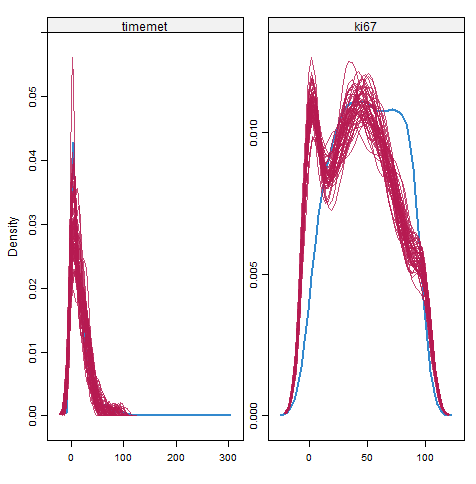
\includegraphics[width=.5\textwidth]{cont_densplot}%
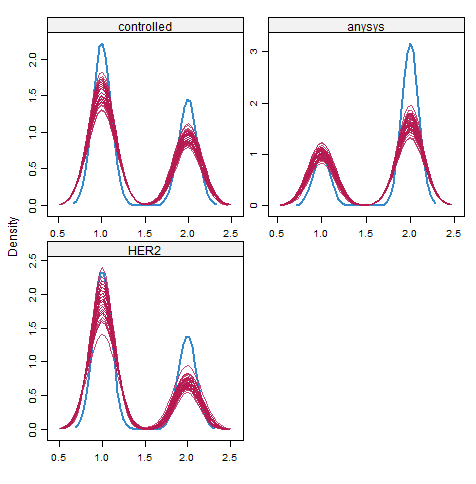
\includegraphics[width=.5\textwidth]{discrete_densplot} 
\end{frame}

%% moved these validity checks to extras

\begin{frame}{MI data Breakdown}
\begin{table}[!ht]
\adjustbox{max height=\dimexpr\textheight-5.5cm\relax,
           max width=\textwidth}{
\centering
\begin{tabular}{|r|c|c|c|c|}
\hline
\multicolumn{1}{|l|}{}                            & \begin{tabular}[c]{@{}c@{}}Sys therapy \\ available case\end{tabular} & \begin{tabular}[c]{@{}c@{}}Sys therapy \\ MI\end{tabular} & \begin{tabular}[c]{@{}c@{}}No Sys therapy \\ available case\end{tabular} & \begin{tabular}[c]{@{}c@{}}No Sys therapy \\ MI\end{tabular} \\ \hline
\multicolumn{1}{|l|}{Age (mean,sd)}               & 51.4(10.8)                                                            & 51.2(10.9)                                                & 52.7(11.9)                                                               & 52.9(11.4)                                                   \\ \hline
\multicolumn{1}{|l|}{Breast Cancer subtype}       &                                                                       &                                                           &                                                                          &                                                              \\ \hline
HR+/HER2-                                         & 27\%                                                                  & 31\%                                                      & 28\%                                                                     & 33\%                                                         \\ \hline
HR+/HER2+                                         & 19\%                                                                  & 18\%                                                      & 12\%                                                                     & 13\%                                                         \\ \hline
HR-/HER2+                                         & 22\%                                                                  & 20\%                                                      & 15\%                                                                     & 12\%                                                         \\ \hline
Triple negative                                   & 32\%                                                                  & 32\%                                                      & 45\%                                                                     & 42\%                                                         \\ \hline
\multicolumn{1}{|l|}{Prior therapies for stage 4} & 1(0-3)                                                                & 2(0-4)                                                    & 2(0-4)                                                                   & 2(0-4)                                                       \\ \hline
\multicolumn{1}{|l|}{Single brain lesion}         & 25\%                                                                  & 23\%                                                      & 23\%                                                                     & 20\%                                                         \\ \hline
\multicolumn{1}{|l|}{Controlled extra-cranial}    & 40\%                                                                  & 40\%                                                      & 35\%                                                                     & 36\%                                                         \\ \hline
\multicolumn{1}{|l|}{ECOG 0-1}                    & 84\%                                                                  & 70\%                                                      & 53\%                                                                     & 40\%                                                         \\ \hline
\multicolumn{1}{|l|}{Local Therapy}               &                                                                       &                                                           &                                                                          &                                                              \\ \hline
Resection Alone                                   & 5\%                                                                   & 5\%                                                       & 9\%                                                                      & 7\%                                                          \\ \hline
SBRT alone                                        & 13\%                                                                  & 12\%                                                      & 9\%                                                                      & 8\%                                                          \\ \hline
WBRT                                              & 60\%                                                                  & 59\%                                                      & 52\%                                                                     & 53\%                                                         \\ \hline
Resection/SBRT+WBRT                               & 12\%                                                                  & 14\%                                                      & 10\%                                                                     & 8\%                                                          \\ \hline
no local therapy                                  & 10\%                                                                  & 10\%                                                      & 20\%                                                                     & 23\%                                                         \\ \hline
\end{tabular}
}
\caption{Characteristics of available case data versus MI data}
\label{table:chartab}
\end{table}
 
\end{frame}










%%%
\begin{frame}{Chemo KM and Log Rank Test}
  \begin{columns}[onlytextwidth]
    \begin{column}{0.75\textwidth}
	 \begin{figure}[h!]
  \centering
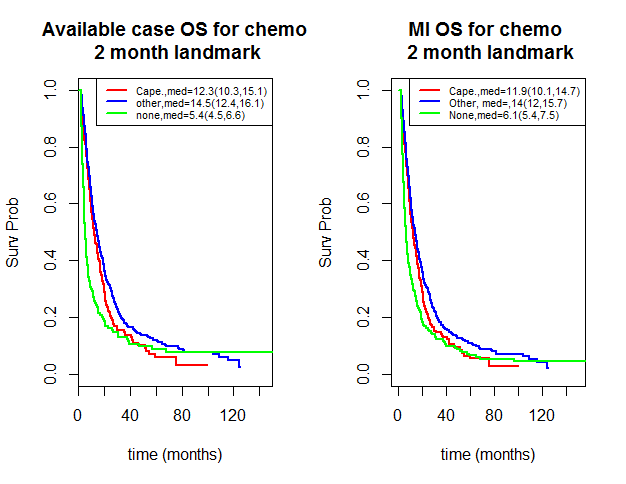
\includegraphics[width=.99\textwidth]{cape_km}
\end{figure}

    \end{column}
    \begin{column}{0.25\textwidth}
    \begin{table}[]
\centering
\adjustbox{max height=\dimexpr\textheight-5.5cm\relax,
           max width=\textwidth}{
\begin{tabular}{|l|c|c|}
\hline
                & \multicolumn{2}{c|}{Chemo}                         \\ \hline
                & \multicolumn{1}{l|}{AC} & \multicolumn{1}{l|}{MI} \\ \hline
cape/other/none & \textless.0001          & \textless.0001          \\ \hline
cape/other      & 0.0321                  & 0.033                   \\ \hline
cape/none       & 0.00039                 & .0016                   \\ \hline
other/none      & \textless.0001          & \textless.0001          \\ \hline
\end{tabular}
}
\end{table}

    \end{column}

	\end{columns}
\end{frame}



\begin{frame}{HER2 Directed KM and Log Rank Test}
  \begin{columns}[onlytextwidth]
    \begin{column}{0.75\textwidth}
	 \begin{figure}[h!]
  \centering
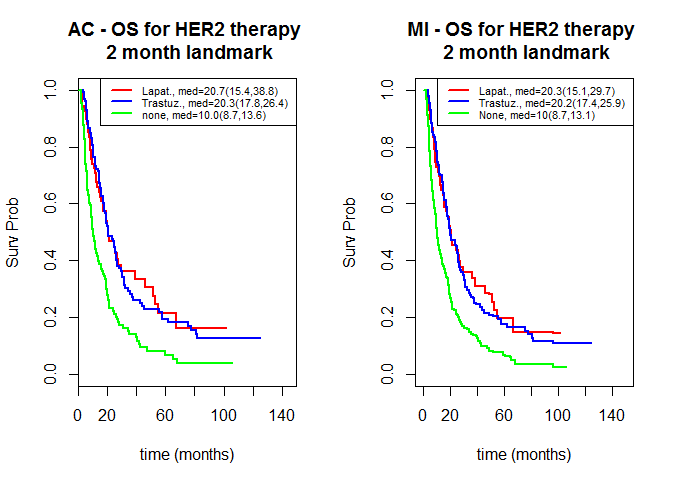
\includegraphics[width=.99\textwidth]{lapat_km}
\end{figure}

    \end{column}
    \begin{column}{0.25\textwidth}
    \begin{table}[]
\centering
\adjustbox{max height=\dimexpr\textheight-5.5cm\relax,
           max width=\textwidth}{
\begin{tabular}{|l|c|c|}
\hline
                   & \multicolumn{2}{c|}{HER2}                         \\ \hline
                   & \multicolumn{1}{l|}{AC} & \multicolumn{1}{l|}{MI} \\ \hline
Lapat/Traztuz/none & \textless.0001          & \textless.0001          \\ \hline
Lapat/Trastuz      & .87                     & .81                     \\ \hline
Lapat/none         & .00017                  & .00018                  \\ \hline
Trastuz/none       & \textless.0001          & \textless.0001          \\ \hline
\end{tabular}
}
\end{table}

    \end{column}

	\end{columns}
\end{frame}


\begin{comment}

\begin{frame}{Kaplan-Meier in MI}
 \begin{itemize}
  \item Non-informative censoring reasonable
  \item Pooled by Rubin's Rules on Complimentary log-log
 \end{itemize}
 \begin{figure}[h!]
  \centering
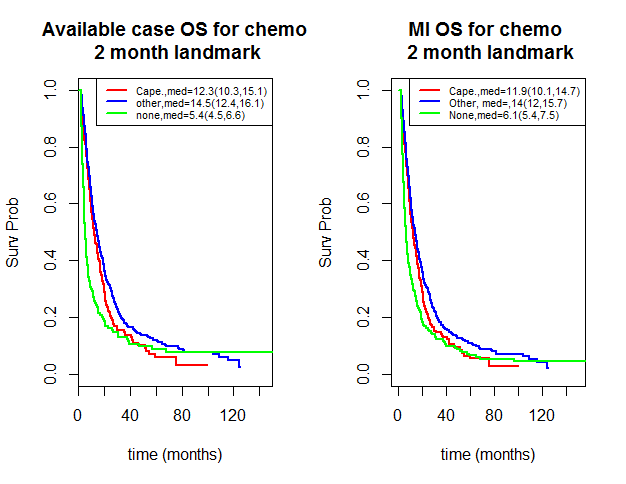
\includegraphics[width=.75\textwidth]{cape_km}
\end{figure}




\end{frame}




\begin{frame}{Kaplan-Meier in MI}
 \begin{figure}[h!]
  \centering
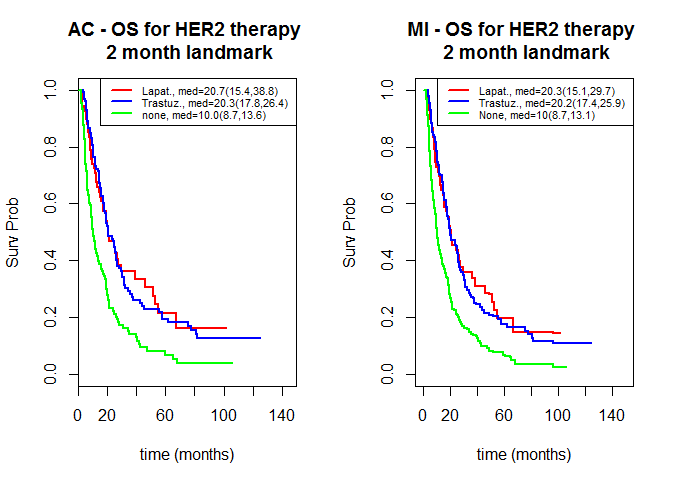
\includegraphics[width=.8\textwidth]{lapat_km}
\end{figure}
 
\end{frame}

\begin{frame}{Log Rank Test}
!!! Will want to combine this with km plots
\begin{table}[]
\centering
\begin{tabular}{|l|c|c|}
\hline
                & \multicolumn{2}{c|}{Chemo}                         \\ \hline
                & \multicolumn{1}{l|}{AC} & \multicolumn{1}{l|}{MI} \\ \hline
cape/other/none & \textless.0001          & \textless.0001          \\ \hline
cape/other      & 0.0321                  & 0.033                   \\ \hline
cape/none       & 0.00039                 & .0016                   \\ \hline
other/none      & \textless.0001          & \textless.0001          \\ \hline
\end{tabular}
\end{table}
%
\begin{table}[]
\centering
\adjustbox{max height=\dimexpr\textheight-5.5cm\relax,
           max width=\textwidth}{
\begin{tabular}{|l|c|c|}
\hline
                   & \multicolumn{2}{c|}{HER2}                         \\ \hline
                   & \multicolumn{1}{l|}{AC} & \multicolumn{1}{l|}{MI} \\ \hline
Lapat/Traztuz/none & \textless.0001          & \textless.0001          \\ \hline
Lapat/Trastuz      & .87                     & .81                     \\ \hline
Lapat/none         & .00017                  & .00018                  \\ \hline
Trastuz/none       & \textless.0001          & \textless.0001          \\ \hline
\end{tabular}
}
\end{table}
\end{frame}

 
\begin{frame}{Cox Model in MI}
\begin{itemize}
 \item Get good baseline model
 \item Need to check proportional hazards
 \item Add treatment variables
\end{itemize}
\end{frame}

\end{comment}

\begin{frame}{Schoenfeld Residual Splines}
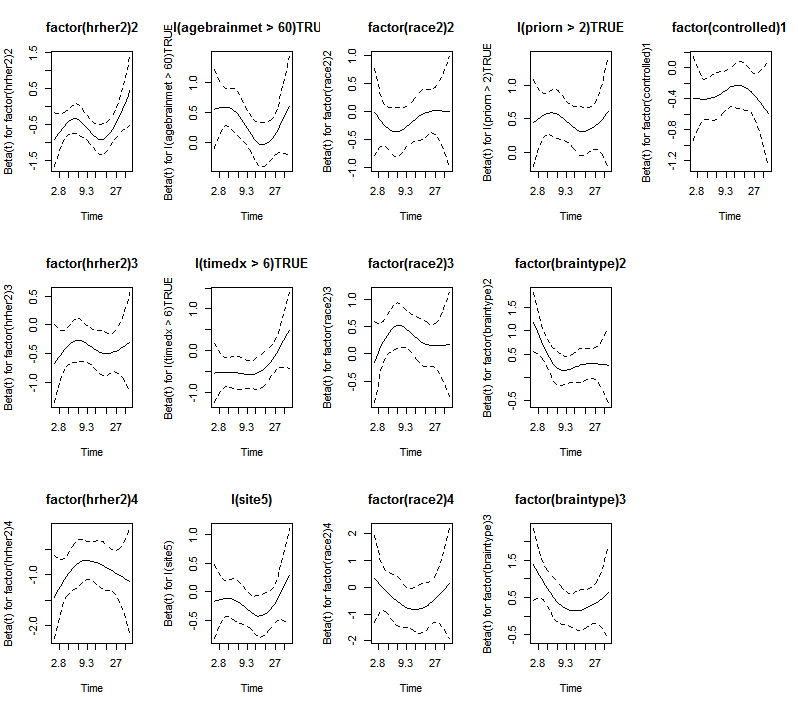
\includegraphics[width=.5\textwidth]{ac_schoenfeld}%
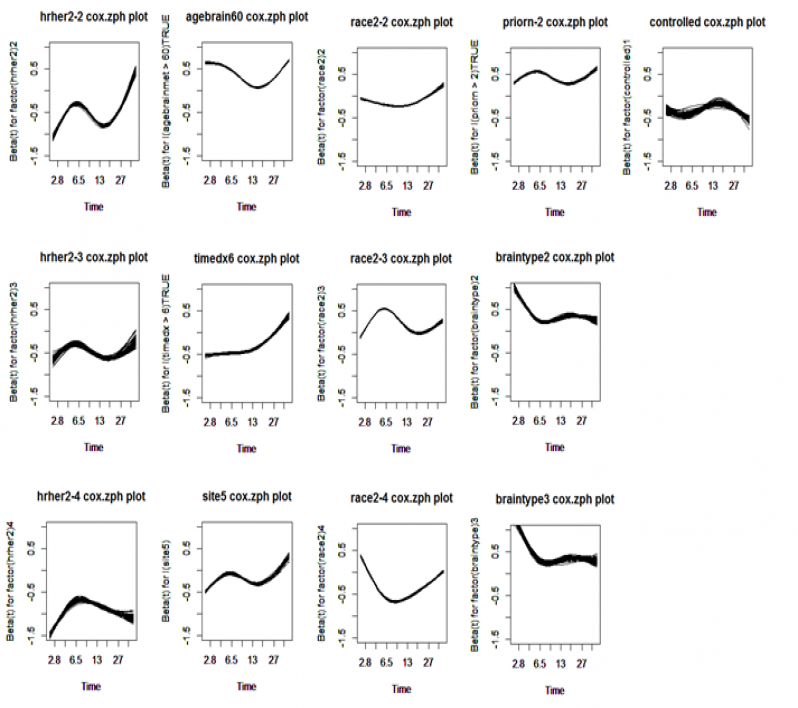
\includegraphics[width=.5\textwidth]{mi_schoenfeld} 
\end{frame}

\begin{frame}{Base model}
 \begin{table}[]
\centering
\adjustbox{max height=\dimexpr\textheight-5.5cm\relax,
           max width=\textwidth}{
\begin{tabular}{|c|c|c|c|c|c|c|c|c|}
\hline
                                                       &                                  &      & \begin{tabular}[c]{@{}c@{}}AC \\ n= 845\end{tabular} &                 &  &      & MI                                                 &                                                            \\ \hline
Variable                                               & Contrast                         & HR   & \begin{tabular}[c]{@{}c@{}}95\% \\ CI\end{tabular}   & pvalue          &  & HR   & \begin{tabular}[c]{@{}c@{}}95\% \\ CI\end{tabular} & \begin{tabular}[c]{@{}c@{}}pvalue\\  (t test)\end{tabular} \\ \hline
HR/HER2                                                & -/+ vs. -/-                      & 0.57 & (0.46,0.71)                                          & \textless0.0001 &  & 0.59 & (0.48,0.72)                                        & \textless0.0001                                            \\ \hline
                                                       & +/- vs. -/-                      & 0.66 & (0.54,0.81)                                          & \textless0.0001 &  & 0.63 & (0.52,0.76)                                        & \textless0.0001                                            \\ \hline
                                                       & +/+ vs. -/-                      & 0.4  & (0.31,0.50)                                          & \textless0.0001 &  & 0.4  & (0.32,0.50)                                        & \textless0.0001                                            \\ \hline
Age                                                    & \textgreater 60 vs. \textless 60 & 1.37 & (1.13,1.65)                                          & 0.0011          &  & 1.45 & (1.22,1.72)                                        & \textless0.0001                                            \\ \hline
Dx to BM                                               & \textgreater 6 vs. \textless 6   & 0.66 & (0.54,0.82)                                          & 0.00013         &  & 0.71 & (0.59,0.86)                                        & 0.0002                                                     \\ \hline
First DM                                               & Brain vs. Oth                    & 0.8  & (0.66,0.97)                                          & 0.026           &  & 0.83 & (0.70,0.99)                                        & 0.02                                                       \\ \hline
Race                                                   & Hisp. Vs. White                  & 0.85 & (0.68,1.07)                                          & 0.17            &  & 0.88 & (0.71,1.08)                                        & 0.11                                                       \\ \hline
                                                       & Black vs. White                  & 1.31 & (1.06,1.63)                                          & 0.014           &  & 1.25 & (1.02,1.52)                                        & 0.015                                                      \\ \hline
                                                       & Other vs. White                  & 0.65 & (0.40,1.04)                                          & 0.075           &  & 0.7  & (0.45,1.07)                                        & 0.05                                                       \\ \hline
\begin{tabular}[c]{@{}c@{}}\# prior \\ Rx\end{tabular} & \textgreater2 vs. 0-2            & 1.58 & (1.31,1.91)                                          & \textless0.0001 &  & 1.53 & (1.29,1.82)                                        & \textless0.0001                                            \\ \hline
BM type                                                & Mult. Vs. Single                 & 1.45 & (1.20,1.76)                                          & \textless0.0001 &  & 1.48 & (1.24,1.76)                                        & \textless0.0001                                            \\ \hline
                                                       & LMD vs. Single                   & 1.6  & (1.21,2.13)                                          & 0.001           &  & 1.58 & (1.25,2.00)                                        & \textless0.0001                                            \\ \hline
Sys. Cont.                                             & Yes vs. No                       & 0.71 & (0.61,0.83)                                          & \textless0.0001 &  & 0.73 & (0.63,0.85)                                        & \textless0.0001                                            \\ \hline
\end{tabular}
}
\caption{AC and MI baseline Cox model}
\label{fig:acmicox}
\end{table}

\end{frame}

\begin{frame}{MI Cox Model, Chemo}
\begin{table}[]
\centering
\adjustbox{max height=.9\dimexpr\textheight-5.5cm\relax,
           max width=\textwidth}{
\begin{tabular}{|l|l|c|c|c|c|c|c|c|}
\hline
                               &                                  &  &  \begin{tabular}[c]{@{}c@{}}AC\\ n= 745\end{tabular}& \multicolumn{1}{l|}{} & \multicolumn{1}{l|}{} & \multicolumn{1}{l|}{} & MI          & \multicolumn{1}{l|}{}                                       \\ \hline
\multicolumn{1}{|c|}{Variable} & \multicolumn{1}{c|}{Contrast}    & HR                                                  & 95\% CI               & p-value               & \multicolumn{1}{l|}{} & HR                    & 95\% CI     & \begin{tabular}[c]{@{}c@{}}p-value \\ (t test)\end{tabular} \\ \hline
HR/HER2                        & -/+ vs. -/-                      & 0.62                                                & (0.49,0.79)           & \textless .0001       &                       & 0.63                  & (0.51,0.77) & \textless .0001                                             \\ \hline
                               & +/- vs. -/-                      & 0.65                                                & (0.53,0.81)           & 0.00011               &                       & 0.64                  & (0.53,0.78) & \textless .0001                                             \\ \hline
                               & +/+ vs. -/-                      & 0.41                                                & (0.31,0.53)           & \textless .0001       &                       & 0.42                  & (0.34,0.53) & \textless .0001                                             \\ \hline
Age                            & \textgreater 60 vs. \textless 60 & 1.34                                                & (1.10,1.64)           & 0.0041                &                       & 1.44                  & (1.21,1.72) & \textless .0001                                             \\ \hline
Dx to BM                       & \textgreater 6 vs. \textless 6   & 0.72                                                & (0.58,0.90)           & 0.0032                &                       & 0.71                  & (0.58,0.86) & 0.00039                                                     \\ \hline
First DM                       & Brain vs. Oth                    & 0.77                                                & (0.63,0.95)           & 0.014                 &                       & 0.81                  & (0.68,0.96) & 0.016                                                       \\ \hline
Race                           & Hisp. Vs. White                  & 0.77                                                & (0.61,0.98)           & 0.034                 &                       & 0.86                  & (0.69,1.06) & 0.15                                                        \\ \hline
                               & Black vs. White                  & 1.29                                                & (1.02,1.63)           & 0.032                 &                       & 1.23                  & (1.01,1.51) & 0.043                                                       \\ \hline
                               & Other vs. White                  & 0.76                                                & (0.47,1.25)           & 0.28                  &                       & 0.7                   & (0.45,1.08) & 0.11                                                        \\ \hline
\# prior Rx                    & \textgreater2 vs. 0-2            & 1.61                                                & (1.32,1.98)           & \textless .0001       &                       & 1.53                  & (1.28,1.82) & \textless .0001                                             \\ \hline
BM type                        & Mult. Vs. Single                 & 1.46                                                & (1.20,1.78)           & 0.00017               &                       & 1.51                  & (1.27,1.81) & \textless .0001                                             \\ \hline
                               & LMD vs. Single                   & 1.45                                                & (1.04,2.03)           & 0.029                 &                       & 1.41                  & (1.11,1.80) & 0.0049                                                      \\ \hline
Sys. Cont.                     & Yes vs. No                       & 0.57                                                & (0.48,0.68)           & \textless .0001       &                       & 0.69                  & (0.59,0.80) & \textless .0001                                             \\ \hline
Chemo                          & Cape. vs. none                   & 0.69                                                & (0.53,0.89)           & 0.0046                &                       & 0.75                  & (0.60,0.95) & 0.018                                                       \\ \hline
                               & other vs. none                   & 0.52                                                & (0.42,0.65)           & \textless .0001       &                       & 0.58                  & (0.47,0.71) & \textless .0001                                             \\ \hline
\end{tabular}
}
\caption{AC and MI Cox model with Chemo Treatment}
\label{acmi_cox_chemo}
\end{table} 
\end{frame}

\begin{frame}{AC and MI Cox Model with HER2 Treatment}
\begin{table}[]
\centering
\adjustbox{max height=\dimexpr\textheight-5.5cm\relax,
           max width=\textwidth}{
\begin{tabular}{|l|l|c|c|c|c|c|c|c|}
\hline
                               &                                  & \multicolumn{1}{l|}{} & \begin{tabular}[c]{@{}c@{}}AC\\ n=292\end{tabular} & \multicolumn{1}{l|}{} & \multicolumn{1}{l|}{} &      & \begin{tabular}[c]{@{}c@{}}MI\\ n between 391\\ and 415\end{tabular} & \multicolumn{1}{l|}{}                                       \\ \hline
\multicolumn{1}{|c|}{Variable} & \multicolumn{1}{c|}{Contrast}    & HR                    & 95\% CI                                            & p-value               &                       & HR   & 95\% CI                                                              & \begin{tabular}[c]{@{}c@{}}p-value \\ (t test)\end{tabular} \\ \hline
HR/HER2                        & +/+ vs. -/+                      & 0.65                  & (0.49,0.87)                                        & 0.0036                &                       & 0.66 & (0.51,0.85)                                                          & 0.0015                                                      \\ \hline
Age                            & \textgreater 60 vs. \textless 60 & 1.38                  & (0.95,2.01)                                        & 0.092                 &                       & 1.58 & (1.15,2.18)                                                          & 0.0054                                                      \\ \hline
Dx to BM                       & \textgreater 6 vs. \textless 6   & 0.64                  & (0.43,0.97)                                        & 0.033                 &                       & 0.69 & (0.49,0.99)                                                          & 0.041                                                       \\ \hline
First DM                       & Brain vs. Oth                    & 0.84                  & (0.58,1.20)                                        & 0.34                  &                       & 0.86 & (0.62,1.17)                                                          & 0.34                                                        \\ \hline
Race                           & Hisp. Vs. White                  & 0.69                  & (0.46,1.02)                                        & 0.064                 &                       & 0.76 & (0.53,1.09)                                                          & 0.14                                                        \\ \hline
                               & Black vs. White                  & 1.41                  & (0.94,2.11)                                        & 0.1                   &                       & 1.43 & (1.00,2.04)                                                          & 0.047                                                       \\ \hline
                               & Other vs. White                  & 0.7                   & (0.32,1.53)                                        & 0.38                  &                       & 0.83 & (0.46,1.52)                                                          & 0.55                                                        \\ \hline
\# prior Rx                    & \textgreater2 vs. 0-2            & 1.88                  & (1.34,2.63)                                        & 0.00028               &                       & 1.71 & (1.28,2.28)                                                          & 0.00028                                                     \\ \hline
BM type                        & Mult. Vs. Single                 & 1.3                   & (0.92,1.86)                                        & 0.14                  &                       & 1.25 & (0.91,1.70)                                                          & 0.16                                                        \\ \hline
                               & LMD vs. Single                   & 2.15                  & (1.20,3.88)                                        & 0.011                 &                       & 1.77 & (1.10,2.83)                                                          & 0.018                                                       \\ \hline
Sys. Cont.                     & Yes vs. No                       & 0.73                  & (0.55,0.97)                                        & 0.029                 &                       & 0.78 & (0.60,1.01)                                                          & 0.063                                                       \\ \hline
HER2 therapy                   & Lapat vs. none                   & 0.47                  & (0.32,0.69)                                        & 0.00015               &                       & 0.52 & (0.37,0.75)                                                          & 0.00036                                                     \\ \hline
                               & Trastuz vs. none                 & 0.45                  & (0.33,0.61)                                        & \textless.0001        &                       & 0.51 & (0.38,0.68)                                                          & \textless.0001                                              \\ \hline
\end{tabular}
}
\caption{AC and MI Cox model with HER2 Treatment}

\end{table}
\end{frame}

\begin{frame}{Causal Analysis}
\begin{itemize}
 \item Need to get propensity score from \textit{pretreatment} covariates
 \item Check the balance and standardized bias
 \item Run IPTW analysis on each dataset
 \item Use Mitra and Reiter's within method to get each MI dataset ATE \cite{Mitra2012}
 \item Pool via Rubin's Rules
\end{itemize}
\end{frame}

 
%causal issues were here


\begin{frame}{IPTW Weighting in MI Setting}
\begin{itemize}
 \item Set the propensity score model - GBM
 \begin{itemize}
  \item Confounding factors: stage, race, IDC, breast cancer surgery, HR/HER2 status,
  breast cancer radiation, first met site, number of prior treatments, ECOG score,
  localized brain mets treatment, age at brain met, type of brain mets, brain met controlled
 \end{itemize}

 \item Weight observations by propensity score
 \item Check to ensure balance achieved -KS and standardized bias
 \item Run IPTW weighted Cox regression on treatment
 \item Pool results via Rubin's rules
 %\item Double robustness: Include pretreatment variables in model?
\end{itemize} 
\end{frame}


\begin{frame}{Balance Checks}
  \begin{figure}[h!]
  \centering
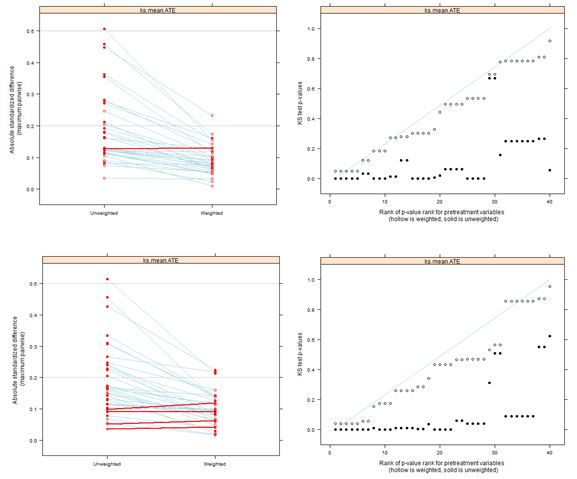
\includegraphics[width=.8\textwidth]{balance_diagnosis} 
  \caption{Selected Balance Diagnostics}
\label{fig:balcheck}
\end{figure}

\end{frame}

\begin{frame}{Results of IPTW: Chemotherapeutic}
 \begin{table}[]
\centering
\adjustbox{max height=\dimexpr\textheight-5.5cm\relax,
           max width=\textwidth}{
\begin{tabular}{|c|c|c|c|c|c|c|c|c|c|c|c|}
\hline
               & \multicolumn{2}{c|}{AC Unweighted} &  & \multicolumn{2}{c|}{AC IPTW} &  & \multicolumn{2}{c|}{MI unweighted} &  & \multicolumn{2}{c|}{MI IPTW} \\ \hline
               & HR           & 95\% CI             &  & HR        & 95\% CI          &  & HR           & 95\% CI             &  & HR         & 95\% CI         \\ \hline
Cape. vs none  & 0.396        & (0.325,0.482)       &  & 0.655     & (0.481,0.894)    &  & 0.484        & (0.400,0.585)       &  & 0.702          & (0.543,0.906)           \\ \hline
Other vs none  & 0.336        & (0.287,0.394)       &  & 0.567     & (0.46,0.754)     &  & 0.413        & (0.354,0.481        &  & 0.593          & (0.470,0.748)           \\ \hline
Cape. vs other & 1.179        & (0.983,1.416)       &  & 1.156     & (0.966,1.383)    &  & 1.173        & (0.981,1.402)       &  & X          & (Y,Z)           \\ \hline
\end{tabular}
}
\caption{Chemotherapeutic ATE with IPTW weights, AC and MI}

\end{table}


 !! Need to put in doubly robust table here!!!
\end{frame}

\begin{frame}{Results of IPTW: HER2 Directed}

\begin{table}[]
\centering
\adjustbox{max height=\dimexpr\textheight-5.5cm\relax,
           max width=\textwidth}{
\begin{tabular}{|l|c|c|c|c|c|c|c|c|c|c|c|}
\hline
                   & \multicolumn{2}{c|}{AC Unweighted}                              & \multicolumn{1}{l|}{} & \multicolumn{2}{c|}{AC IPTW}                                    & \multicolumn{1}{l|}{} & \multicolumn{2}{c|}{MI Unweighted}                              & \multicolumn{1}{l|}{} & \multicolumn{2}{c|}{MI IPTW}                                    \\ \hline
                   & HR                         & 95\% CI                            &                       & HR                         & 95\% CI                            &                       & HR                         & 95\% CI                           &                       & HR                         & 95\% CI                            \\ \hline
Lapat. vs none     & 0.467                      & (0.355,0.616)                      &                       & 0.571                      & (0.381,0.855)                      &                       & 0.474                      & (0.362,0.622)                     &                       & 0.485                      & (0.304,0.775)                      \\ \hline
Trastuz. vs none   & 0.488                      & (0.398,0.597)                      &                       & 0.566                      & (0.421,0.759)                      &                       & 0.506                      & (0.417,0.614)                     &                       & 0.480                      & (0.313,0.735)                      \\ \hline
Lapat. vs Trastuz. & \multicolumn{1}{l|}{0.958} & \multicolumn{1}{l|}{(0.693,1.324)} & \multicolumn{1}{l|}{} & \multicolumn{1}{l|}{1.009} & \multicolumn{1}{l|}{(0.680,1.496)} & \multicolumn{1}{l|}{} & \multicolumn{1}{l|}{0.927} & \multicolumn{1}{l|}{(0.673,1.28)} & \multicolumn{1}{l|}{} & \multicolumn{1}{l|}{1.011} & \multicolumn{1}{l|}{(0.763,1.338)} \\ \hline
\end{tabular}
}
\caption{HER2 directed ATE with IPTW weights, AC and MI}
\label{tab:lapatonly}
\end{table}

\begin{table}[]
\centering
\adjustbox{max height=\dimexpr\textheight-5.5cm\relax,
           max width=\textwidth}{
\begin{tabular}{|c|c|c|c|c|c|c|c|c|c|c|c|}
\hline
                   & \multicolumn{2}{c|}{AC Unweighted} &  & \multicolumn{2}{c|}{AC IPTW} &  & \multicolumn{2}{c|}{MI Unweighted} &  & \multicolumn{2}{c|}{MI IPTW} \\ \hline
                   & HR          & 95\% CI              &  & HR        & 95\% CI          &  & HR           & 95\% CI             &  & HR         & 95\% CI            \\ \hline
Lapat. vs none     & 0.468       & (0.316,0.692)        &  & 0.514     & (0.331,0.798)    &  & 0.524        & (0.367,0.747)       &  & 0.410      & (0.257,0.652)      \\ \hline
Trastuz. vs none   & 0.447       & (0.328,0.6089)       &  & 0.456     & (0.328,0.632)    &  & 0.511        & (0.381,0.685)       &  & 0.388      & (0.249,0.602)      \\ \hline
Lapat. vs Trastuz. & 1.048       & (0.704,1.560)        &  & 1.128     & (0.726,1.754)    &  & 1.026        & (0.713,1.477)       &  & 1.057      & (0.788,1.417)      \\ \hline
\end{tabular}
}
\caption{HER2 directed ATE with IPTW weights, double robust}
\label{lapatfull}
\end{table}
 
\end{frame}

